\chapter{Walking Straight}
\label{chap:intro}

\section{Introduction}

\label{sec:xrefs}

A well-known problem associated with walking without vision is veering, which is the inability to maintain a straight path. Many studies conducted previously have proven the veering effect and its consequences. The reason is uncertain but is hypothesized to be motor error in stepping movement.  Blind people face the same problem while walking. This makes crossing intersections and walking on a straight path dangerous and unsafe.

‘Walking Straight’ an application for the smartphone device was built by Paneels et al. \cite{walkingstraight}. It uses the available hardware on a smartphone device, the iPhone 4, to provide real-time audio feedback to the blind users in order to correct their deviation. The application is built using the ISAS (In-Situ Audio Services) \cite{BlumMonet} system architecture. The application uses compass and gyroscope sensors to calculate the deviation from a straight path. The values from the sensors are filtered to remove body sway of a person while walking. Different auditory feedback designs were evaluated experimentally and their performance was evaluated. A continuous tone played in the ear in the side of the deviation is concluded to be the most efficient way of rendering the audio feedback to the blind \cite{walkingstraight}.

\section{Are the sensors reliable?}

The study of today’s smartphone sensors’ reliability was done by Blum et al.[4]. The current state of the walking straight algorithm assumes a stable 10Hz Gyroscope. It solely depends on the sensors to calculate the heading.  



%natwidth=941,natheight=726
\begin{figure}
\begin{center}
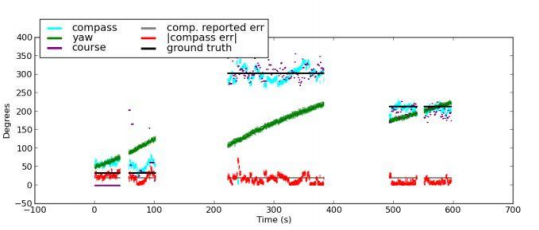
\includegraphics[scale=0.8]{sensor.png}
\caption{Sensor values over time from a single log file.}
\label{fig:sensors}
\end{center}
\end{figure}


Figure~\ref{fig:sensors} indicates compass values (cyan) against ground truth (black), the latter of which is constant (horizontal) for each straight-line leg of the walk. Actual compass error (red) is calculated as the absolute difference between these two, whereas reported compass error (grey) is an estimate of error magnitude by the sensor itself. As ican be seen, the actual error fluctuates both above and below the estimate. Gaps in the plot represent transitions between legs of the walk, during which we have no ground truth heading information.

Yaw (green), obtained from the gyroscope sensor, is not calibrated to north, so this only represents relative variation. This data is should be a flat line, excepting body sway while walking. Slope in yaw indicates drift, observed in all legs of this walk. The reported course (purple) is derived from the direction of travel based on previous location updates. Both the iPhone and Android devices report course and speed based on location changes, but these appear to be of limited use even in the constrained straight-line testing they performed [4]. The inaccurate results of this study indicate that the application cannot solely rely on these sensors \cite{BlumSensors}.

\section{Computer vision solution}
I have been working on overcoming the sensor inaccuracies, using computer vision techniques on the video captured from a smartphone camera, to generate a better feedback for the blind than what is present currently.

\subsection{Problem}
Two kinds of feedback are required by blind people to cross the intersection: when to cross and audio feedback to maintain a straight path. The correct time to cross the street can be determined by the state of the traffic light. The traffic light recognition can be done using color segmentation, shape segmentation or template matching or a combination of these. 

\subsection{Colour Segmentation}
\begin{figure}
\begin{center}
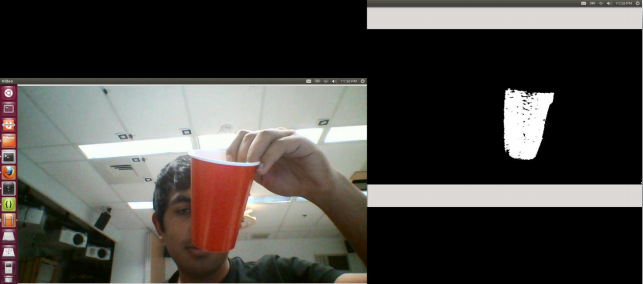
\includegraphics[scale=0.5]{binary.png}
\caption{Conversion into a binary image. Object is Red Cup.}
\label{fig:binary}
\end{center}
\end{figure}
Color Segmentation is the technique to partition an image into different sets of pixels. This can be done using the specific color of the object we want to identify in the frame. I used OpenCV 2.4 to achieve this. I calculated the Hue, Saturation, and Value (HSV). The image from the source, in RGB format, was converted to HSV and then standard thresholding technique was applied. HSV is a color model based on human vision. The image (right) in Figure~\ref{fig:binary} is the binary image, the red cup being shown with white pixels.
 
\subsubsection{Why HSV rather than RGB?}


\begin{itemize}
	\item The simple answer is that unlike RGB, HSV separates Luma, or the image intensity, from Chroma or the colour information. This is very useful in many applications. For example, if you want to do histogram equalization of a colour image, you probably want to do that only on the intensity component, and leave the colour components alone. Otherwise you will get very strange colours.
	\item In computer vision you often want to separate colour components from intensity for various reasons, such as robustness to lighting changes, or removing shadows.
	
\end{itemize}

Using thresholding only, we can track the traffic light, but that will not be accurate for all cases. There might be a few false detections.

\section{False Detections}

For a relatively simple case, such as a sky background, the color-based recognition method can effectively detect and identify traffic light. For a relatively complex situation, such as an urban environment, false detections will appear easily using the color-based recognition method. The shape-based feature recognition method can effectively reduce the false detections of the color-based feature recognition. But, the different shape characteristic rule has to be created for the different styles of traffic lights. This limits the flexibility of the algorithm. For the recognition method based on template matching, the different styles of traffic light templates also have to be created to realize the recognition of the different style of the traffic light.
\begin{figure}
\begin{center}
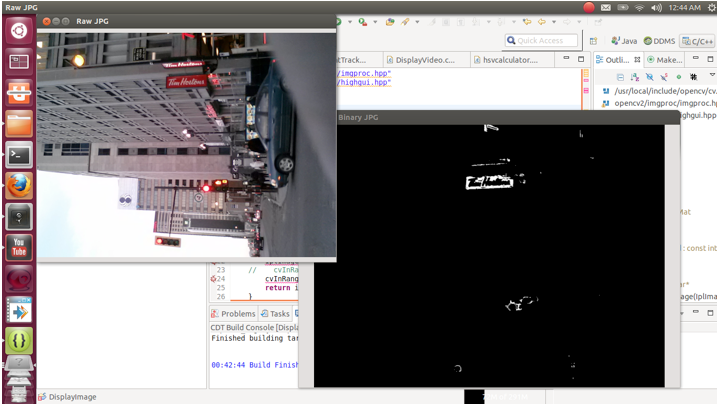
\includegraphics[scale=0.5]{falsede.png}
\caption{False detections in an urban intersection scene.}
\label{fig:falsede}
\end{center}
\end{figure}
\subsection{Region Labelling}
To overcome this problem of false detections in the scene, labeling the candidate region of the traffic light is one of the most feasible solutions. I intend to use the Canny Edge Detector, that is inbuilt in OpenCV libary, which makes it lightweight and efficient. We can detect the closest bounding rectangle of the light and then label the red and green lights accordingly. In this way we can eliminate any other object, which was previously identified as a potential traffic light.  This method was proposed by Gong et al. \cite{gong2010recognition}.

\section{Tracking}
I plan to generate the feedback using OpenCV’s capabilities to extract motion from a video sequence using optical flow. Optical flow assesses motion between two frames without any prior knowledge about the content of the frames. There are two types of tracking techniques, Dense Tracking technique and Sparse Tracking technique. Dense tracking technique utilizes each pixel in the frame to create a motion vector. This is computationally heavy and seldom used nowadays. We will use the Sparse Tracking algorithm which calculates the motion vector for a subset of pixels.
\subsection{CAMShift}
CAMShift is almost ideal for traffic light tracking from a pedestrian's perspective for multiple reasons. One, the speed of the camera (pedestrian) is low. Secondly, the traffic light (object) never disappears from the frame. Camshift allows for tracking objects whose size may change during the sequence. 
\begin{figure}
\begin{center}
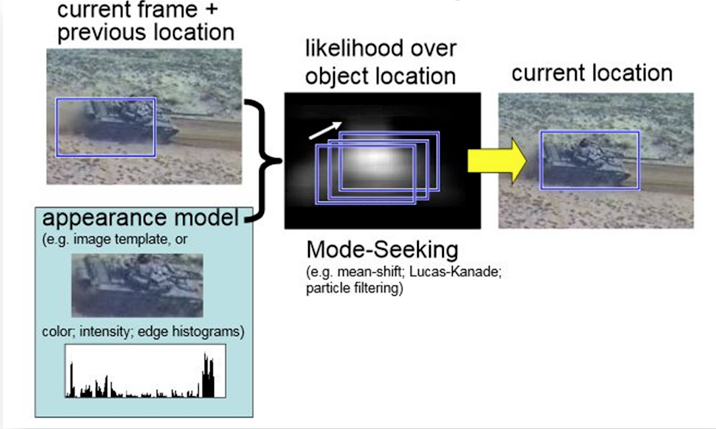
\includegraphics[scale=0.5]{camshift.png}
\caption{CAMShift illustration.}
\label{fig:camshift}
\end{center}
\end{figure}

\section{Future Work}
The larger goal of the algorithm I am building is to help blind people walk straight. Feature extraction from the scene can be used to generate accurate feedback for the blind user. My aim is to find these stable features and train the algorithm to recognize any one of these in the scene. I will implement SIFT and FAST corner detector algorithm for the edge detection. These algorithms are scale and illumination invariant. FAST has been tested on iPhone and is quite efficient. To improve the recognition of state of traffic lights for the pedesrains, the classifier can be trained to recognize the Red Hand Symbol and the numbers below.s




